\vspace{-0.2cm}
\section{Problem Statement, Training Data and Evaluation Protocol}
\label{sec:accel}
\vspace{-0.2cm}
%
Our template-based parameterization maps the accelerator, denoted as $\rvx$, to a discrete design space, $\rvx = [\rvx_1, \rvx_2, \cdots, \rvx_K]$, and each $\rvx_i$ is a discrete-valued variable representing one component of the microarchitectural template, as shown in Table~\ref{tab:arch_params} (See Appendix~\ref{sec:dla_shi_fast} for the description of other accelerator search spaces studied in our work). In our context, the accelerator $\rvx$ plays the same role as an action $\mathbf{a}$.

%
An accelerator design maybe be infeasible due to various reasons, such as a compilation failure or the limitations of physical implementation, and we denote the set of all such feasibility criterion as $\mathrm{Feasible}(\rvx)$. The feasibility criterion depends on both the target software and the underlying hardware, and it is not easy to identify if a given $\rvx$ is infeasible without running explicit simulation. We will require our design procedure to not only learn the value of the objective function but also to learn to navigate through infeasible solutions to performant feasible solutions $\rvx^*$ satisfying $\mathrm{Feasible}(\rvx^*) = 1$. 

Our training dataset $\mathcal{D}$ consists of a modest set of accelerators $\rvx_i$ that are randomly sampled from the design space and evaluated by the hardware simulator. We partition the dataset $\mathcal{D}$ into two subsets, $\mathcal{D}_\text{feasible}$ and $\mathcal{D}_\text{infeasible}$. Let $f(\rvx)$ denote the desired objective (e.g., latency, power, etc.) we intend to optimize over the space of accelerators $\rvx$. We do not possess functional access to $f(\rvx)$, and the optimizer can only access $f(\rvx)$ values for accelerators $\rvx$ in the feasible partition of the data, $\mathcal{D}_\text{feasible}$.
%
For all infeasible accelerators, the simulator does not provide any value of $f(\rvx)$.
In addition to satisfying feasibility, the optimizer must handle explicit constraints on parameters such as area and power~\citep{flynn2011computer}. In our applications, we impose an explicit area constraint, $\mathrm{Area}(\rvx) \leq \review{\alpha_0}$, though additional explicit constraints are also possible. 
%
To account for different constraints, we formulate this task as a constrained optimization problem.
%
Formally:  
\begin{equation}
\label{eqn:opt_prob}
\vspace{-0.2cm}
\begin{aligned}
\min_{\rvx}~ & f(\rvx)
~~~\textrm{s.t.}~~~\mathrm{Area}(\rvx) \leq \review{\alpha_0}, ~~~ \mathrm{Feasible}(\rvx) = 1 \\
\quad &~\text{on}~~ \mathcal{D} = \mathcal{D}_\text{feasible} \cup \mathcal{D}_\text{infeasible} = \{(\rvx_1, \rvy_1), \cdots, (\rvx_N, \rvy_N)\} \cup \{\rvx'_1, \cdots, \rvx'_{N'}\}
\end{aligned}
\end{equation}

While Equation~\ref{eqn:opt_prob} may appear similar to a typical black-box optimization problem, solving it over the space of accelerator designs is challenging due to the large number of infeasible points, the need to handle explicit design constraints, and the difficulty in navigating the non-smooth landscape (See Figure~\ref{fig:ds_dist_all} and Figure~\ref{fig:appx_ds} in the Appendix) of the objective function.
%


\begin{table*}[t!]
\small
\centering
% \vspace*{0.1cm}
\caption{The accelerator design space parameters for the primary accelerator search space targeted in this work. The maximum possible number of accelerator designs (including feasible and infeasible designs) is 452,760,000. \methodname\ only uses a small randomly sampled subset of the search space.}
\label{tab:arch_params}
\vspace{-0.1cm}
\resizebox{0.8\textwidth}{!}{\begin{tabular}{l|l||l|l}
\toprule
\textbf{Accelerator Parameter} &\textbf{\# Discrete Values} & \textbf{Accelerator Parameter} & \textbf{\# Discrete Values}\\\midrule
\# of PEs-X & 10 & \# of PEs-Y & 10\\\hline
PE Memory & 7 & \# of Cores & 7\\\hline
Core Memory & 11 & \# of Compute Lanes & 10\\\hline
Instruction Memory & 4 & Parameter Memory & 5\\\hline
Activation Memory & 7 & DRAM Bandwidth & 6\\
\bottomrule
\end{tabular}}
\vspace{-0.2cm}
\end{table*}

\niparagraph{What makes optimization over accelerators challenging?} Compared to other domains where model-based optimization methods have been applied~\citep{brookes19a,trabucco2021conservative}, optimizing accelerators introduces a number of practical challenges.
%
First, accelerator design spaces typically feature a narrow manifold of feasible accelerators within a sea of infeasible points~\citep{prac_dse:mascots:2019,shi2020learned,gelbart2014bayesian}, as visualized in Figure~\ref{fig:ds_dist_all} and Appendix (Figure~\ref{fig:tsne_infeasible}).
%
While some of these infeasible points can be identified via simple rules (e.g. estimating chip area usage), most infeasible points correspond to failures during compilation or hardware simulation. These infeasible points are generally not straightforward to formulate into the optimization problem and requires simulation~\citep{shi2020learned,timeloop,yazdanbakhsh2021apollo}.

Second, the optimization objective can exhibit high sensitivity to small variations in some architecture parameters (Figure~\ref{fig:appx_ds_memory}) in some regions of the design space, but remain relatively insensitive in other parts, resulting in a complex optimization landscape. This suggests that optimization algorithms based on local parameter updates (e.g., gradient ascent,  evolutionary schemes, etc.) may have a challenging task traversing the nearly flat landscape of the objective, which can lead to poor performance.
\begin{figure}[t]
    \begin{center}
    \begin{minipage}{\linewidth}
    \centering
    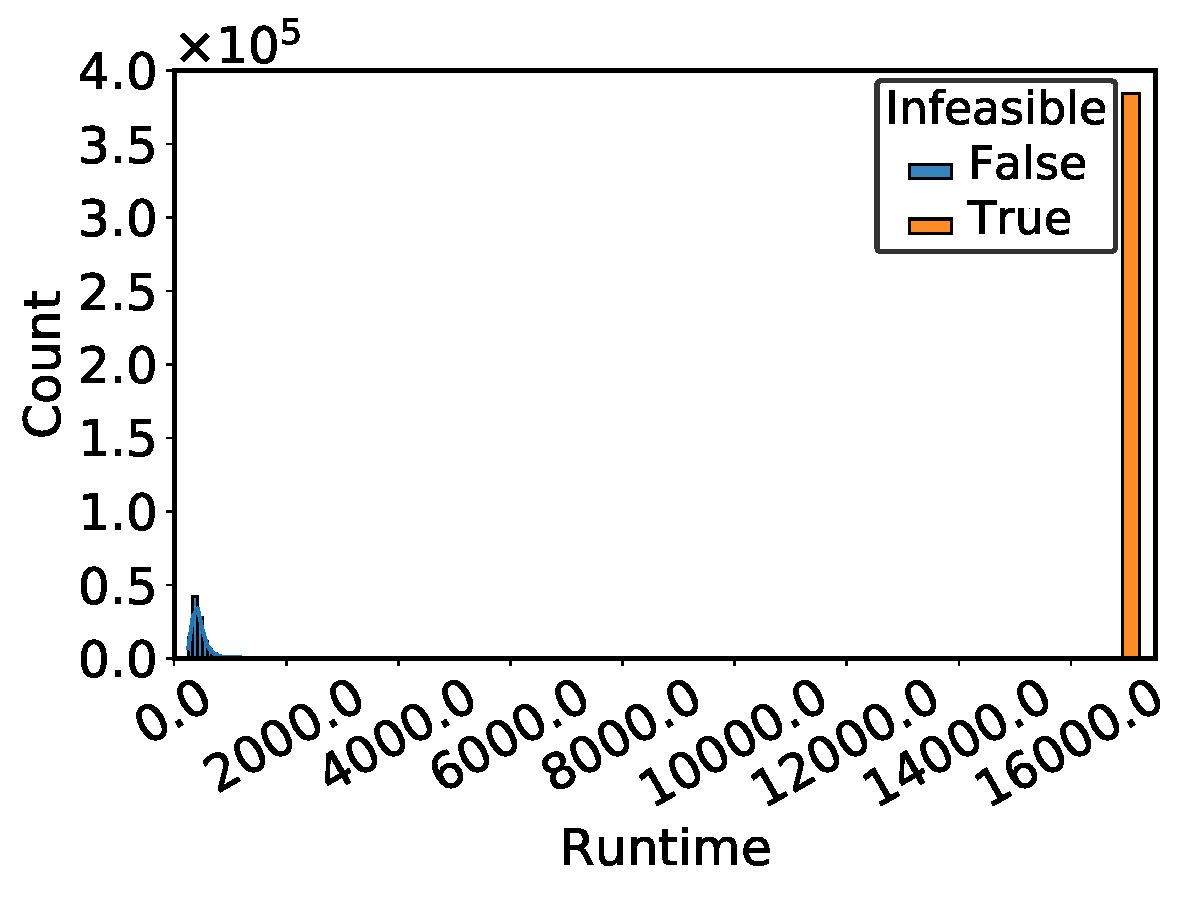
\includegraphics[width=0.35\linewidth]{chapters/prime/figs/dataset/dist.pdf}
    \vspace{-0.1cm}
    \label{fig:ds_dist}
    \centering
    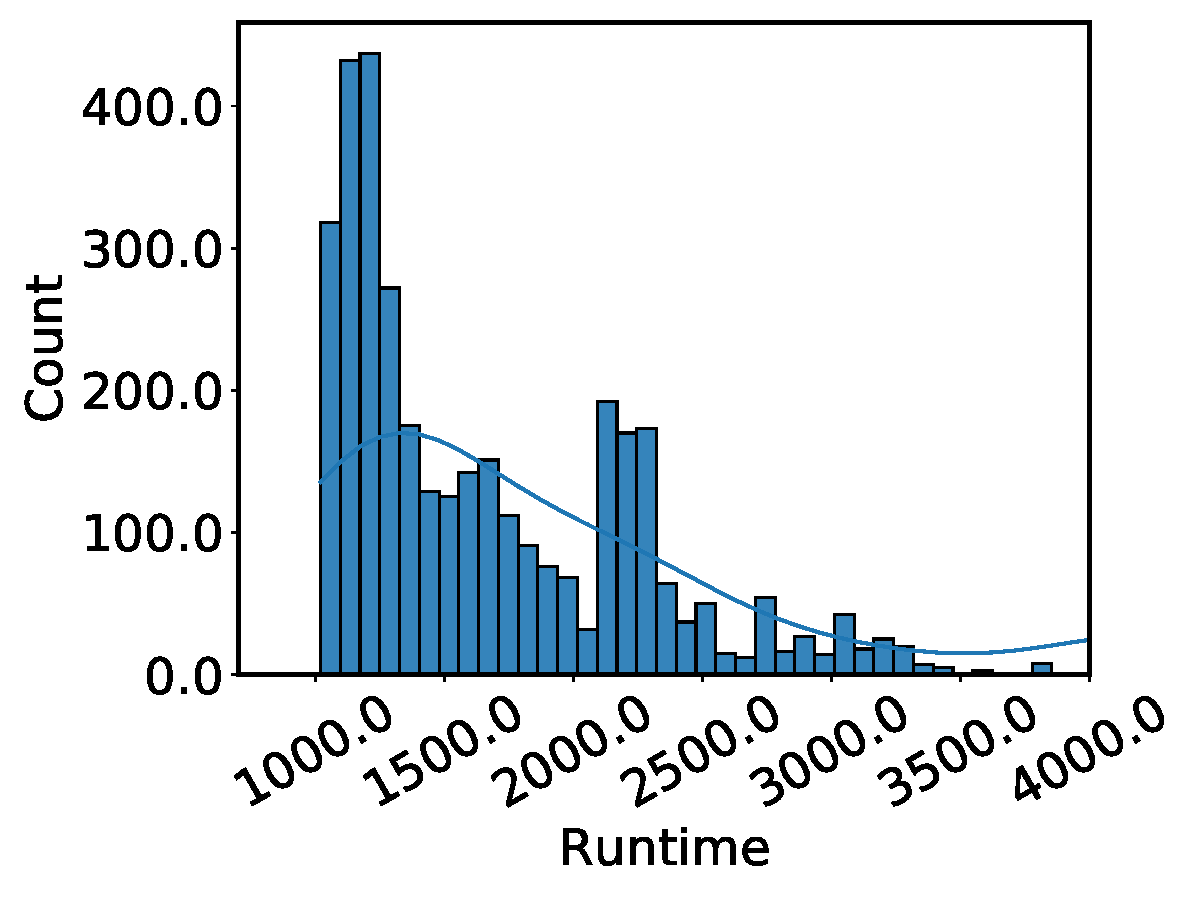
\includegraphics[width=0.35\linewidth]{chapters/prime/figs/dataset/dist_large.pdf}
    \label{fig:ds_dist_large}
    \end{minipage}
    \end{center}
    \vspace{-0.2cm}
    \caption{\footnotesize{\textbf{Left:} histogram of infeasible (right orange bar with large score values) and feasible (left cluster of bars) data points for MobileNetEdgeTPU; \textbf{Right:} zoomed-in histogram (different number of bins) focused on feasible points highlighting the variable latencies.}}
    \vspace{-0.2cm}
    \label{fig:ds_dist_all}
\end{figure}

\niparagraph{Training dataset.}
%
We used an offline dataset $\mathcal{D}$ of (accelerator parameters, latency) via random sampling from the space of 452M possible accelerator configurations.
%
Our method is only provided with a relatively modest set of feasible points ($\leq 8000$ points) for training, and these points are the \emph{worst-performing} feasible points across the pool of randomly sampled data.
%
This dataset is meant to reflect an easily obtainable and an application-agnostic dataset of accelerators that could have been generated once and stored to disk, or might come from real physical experiments. 
%
We emphasize that no assumptions or domain knowledge about the application use case was made during dataset collection.
%
Table~\ref{tab:models} depicts the list of target applications, evaluated in this work, includes three variations of MobileNet~\citep{edgetpu:arxiv:2020,mnv2:arxiv:2018,mnv3:cvpr:2019}, three in-house industry-level models for object detection (M4, M5, M6; names redacted to prevent anonymity violation), a U-net model~\citep{unet}, and two RNN-based encoder-decoder language models~\citep{trnn01,trnn02,trnn03,trnn04}. 
%
These applications span the gamut from small models, such as \msix, with only 0.4~MB model parameters that demands less on-chip memory, to the medium-sized models ($\geq$~5~MB), such as MobileNetV3 and \mfour models, and large models ($\geq$~19~MB), such as t-RNNs, hence requiring larger on-chip memory. 
%
\begin{table*}[h]
\vspace{0.05cm}
\small{
\centering
% \vspace*{0.1cm}
\caption{\footnotesize Description of applications, their domains, number of (convolutions, depth-wise convolutions, feed-forward) XLA ops, model parameter size, instruction sizes in bytes, number of compute operations.}
\label{tab:models}
\vspace{-0.1cm}
\resizebox{\textwidth}{!}{\begin{tabular}{l|l|c|r|r|r}
\toprule
\textbf{Name}&\textbf{Domain}&\textbf{\# of XLA Ops (Conv, D/W, FF)}&\textbf{Model Param}&\textbf{Instr. Size}&\textbf{\# of Compute Ops.}\\\midrule
{\textbf{MobileNetEdgeTPU}} &Image Class.&(45, 13, 1)&3.87~MB&476,736&1,989,811,168\\\hline
{\textbf{MobileNetV2}}&Image Class.&(35, 17, 1)&3.31~MB&416,032&609,353,376\\\hline
{\textbf{MobileNetV3}}&Image Class.&(32, 15, 17)&5.20~MB&1,331,360&449,219,600\\\hline
\textbf{\mfour}&Object Det.&(32, 13, 2)&6.23~MB&317,600&3,471,920,128\\\hline
\textbf{\mfive}&Object Det.&(47, 27, 0)&2.16~MB&328,672&939,752,960\\\hline
\textbf{\msix}&Object Det.&(53, 33, 2)&0.41~MB&369,952&228,146,848\\\hline
\textbf{U-Net}&Image Seg.&(35, 0, 0)&3.69~MB&224,992&13,707,214,848\\\hline
\textbf{t-RNN Dec}&Speech Rec.&(0, 0, 19)&19~MB&915,008&40,116,224\\\hline
\textbf{t-RNN Enc}&Speech Rec.&(0, 0, 18)&21.62~MB&909,696&45,621,248\\
\bottomrule
\end{tabular}}
}
\vspace{-0.25cm}
\end{table*}

\niparagraph{Evaluation protocol.}
%
To compare simulator-driven methods and our data-driven method, we limit the number of feasible points (costly to evaluate) that can be used by any algorithm to equal amounts. We still provide infeasible points to any method and leave it up to the optimization method to use it or not.
This ensures our comparisons are fair in terms of the amount of data available to each method.
However, it is worthwhile to note that in contrast to our method where \emph{worse-quality} data points from small offline dataset are used, the simulator-driven methods have an inherent advantage because they can steer the query process towards the points that are more likely to be better in terms of performance.
Following prior work in data-driven design~\citep{brookes19a}, we evaluate each run of a method by first sampling the top $n=256$ design candidates according to the algorithm's predictions, evaluating all of these under the ground truth objective function and recording the performance of the best accelerator design. The final reported results is the median of ground truth objective values across five independent runs.
